% Provenance (never printed): see sources/outline_sources.md (Year 2: the Himalaya and Tibet;
% the Andes; crustal thickening and plateaus). Himalayan units, thrusts and rates after Lave
% and Avouac (2000), Ader et al. (2012), Cattin et al. (2001), Dong et al. (2026, STDS);
% Asian extrusion after Jiao et al. (2023); Tibetan rifts after Wang et al. (2021); Central
% Andes after Gerbault et al. (2005); flat slabs after Gauthier et al. (2024). Relief from
% ETOPO1 (figdata/bachelor-2/plateaus.py); plate velocities from NNR-MORVEL56 (Book 2 ledger
% row nnr56:poles). Exercise and problem values in the Book 4 scratch calculator
% calc/ch14.py.
\chapter{Cinturões de colisão e cinturões andinos comparados}\label{ch:b2:himalaya-andes}

Dois planaltos na Terra se elevam a mais de quatro quilômetros de altura por centenas de quilômetros.
O Tibete foi soerguido onde a Índia colidiu com a Ásia, dois continentes que se encontraram depois que o oceano entre
eles desapareceu. O Altiplano foi soerguido onde uma placa oceânica, a placa de Nazca, ainda desliza
sob a América do Sul, sem que nenhum continente chegasse. Dois motores diferentes construíram duas
formas de relevo semelhantes. Este capítulo desmonta os dois cinturões, mede quanto sua crosta
se espessou e por quê, e pergunta o que os impede de crescer mais.
% ledger: lave00:setting, gerbault05:andes, data:b4-etopo-tibet, data:b4-etopo-andes

\begin{recall}
\textbf{Do volume do ensino médio}: a colisão continental e a sutura; a deriva da Índia
para o norte, sua desaceleração e a idade debatida da colisão; o Planalto Tibetano, com cerca de
\qty{4600}{m} de altitude sobre uma crosta de cerca de \qty{70}{km} de espessura. \textbf{Do volume do primeiro ano}:
a isostasia de Airy e a placa de Bouguer; as margens ativas, a laje em subducção, o arco vulcânico e
a distância arco--fossa; as velocidades das placas a partir das velocidades angulares; a lei de Byerlee; a magnitude
de momento. \textbf{Do \cref{ch:b2:crustal-melting}}: os \omterm{def:b2:crustal-melting:leucogranite}{leucogranitos} do Himalaia.
\textbf{Do \cref{ch:b2:alpine-orogen}}: \omterm{def:b2:alpine-orogen:orogen}{orógeno}, \omterm{def:b2:alpine-orogen:nappes}{nappe}, \omterm{def:b2:alpine-orogen:decollement}{descolamento}, \omterm{def:b2:alpine-orogen:skin}{tectônica de pele fina} e de
pele grossa, \omterm{def:b2:alpine-orogen:ftb}{cinturão de dobras e cavalgamentos}, \omterm{def:b2:alpine-orogen:foreland}{bacia de antepaís}, \omterm{def:b2:alpine-orogen:balanced}{seções balanceadas}.
\end{recall}

\begin{definition}[Orógeno de colisão; orógeno de tipo andino]\label{def:b2:himalaya-andes:types}
Um \emph{orógeno de colisão}\index{orógeno de colisão} é um \omterm{def:b2:alpine-orogen:orogen}{orógeno} construído pela convergência de
duas margens continentais depois que o oceano entre elas foi consumido; seu eixo é uma sutura.
Um \emph{orógeno de tipo andino}\index{orógeno de tipo andino} é um \omterm{def:b2:alpine-orogen:orogen}{orógeno} construído sobre a placa
cavalgante de uma zona de subducção oceano--continente, enquanto a subducção continua sob ele; seu eixo
é um arco vulcânico.
\end{definition}


\section{A Índia contra a Ásia}\label{sec:b2:himalaya-andes:himalaya}

A Índia encontrou a borda sul da Eurásia há cerca de 50 milhões de anos ao longo da sutura
Indo--Tsangpo, também chamada sutura Indo--Yarlung; a data exata ainda é debatida, como
mostrou o volume do ensino médio. A convergência não parou. Hoje a Índia e a Ásia se aproximam
a cerca de \qty{40}{mm} por ano; pelas velocidades angulares do modelo de placas NNR-MORVEL56, a
Índia se move a \qty{45}{mm} por ano em relação à Eurásia a \ang{28}~N, \ang{85}~L, na direção
\ang{22} a leste do norte. Só parte desse movimento é absorvida no Himalaia. Através do Nepal,
estações GPS mostram a Índia e o sul do Tibete convergindo a $17.8 \pm \qty{0.5}{mm}$ por ano no
centro e no leste e a $20.5 \pm \qty{1}{mm}$ por ano no oeste: cerca da metade do total. O resto
se distribui pelo Tibete e pelo resto da Ásia.
% ledger: lave00:setting, najman21:collision-age, jiao23:extrusion, nnr56:poles, ader12:rates, ader12:mht
% values (plateaus.py): v_india_eurasia 44.99 mm/yr, azimuth 21.65

Os mapas abaixo mostram os dois cinturões com as mesmas curvas de nível, e as faixas ao longo das quais este
capítulo os corta.

\begin{omfigure}
\centering
% ledger: data:b4-etopo-tibet, data:b4-etopo-andes
\begin{tikzpicture}
\begin{axis}[name=tib, scale only axis, width=8.0cm, height=4.8cm, xmin=75, xmax=100,
  ymin=25, ymax=40, xlabel={longitude (\unit{\degree} L)}, ylabel={latitude (\unit{\degree} N)},
  tick label style={font=\scriptsize}, label style={font=\small}, xtick={75,80,...,100},
  ytick={25,30,...,40}, title={\small Himalaia e Tibete}]
\addplot[omThm!35, line width=0.3pt] table[x=lon, y=lat] {figdata/out/bachelor-2-plateaus-tc2000.dat};
\addplot[omThm!90!black, line width=0.4pt] table[x=lon, y=lat] {figdata/out/bachelor-2-plateaus-tc4000.dat};
\draw[black, densely dashed, line width=0.9pt] (axis cs:86,25) rectangle (axis cs:90,40);
\node[font=\scriptsize, fill=white, fill opacity=0.85, text opacity=1, inner sep=1pt] at (axis cs:80,26.2) {planície do Ganges};
\node[font=\scriptsize, fill=white, fill opacity=0.85, text opacity=1, inner sep=1pt] at (axis cs:94.5,33.5) {Planalto Tibetano};
\node[font=\scriptsize, fill=white, fill opacity=0.85, text opacity=1, inner sep=1pt] at (axis cs:83,39.2) {Tarim};
\end{axis}
\begin{axis}[at={(tib.east)}, anchor=west, xshift=1.6cm, scale only axis, width=3.6cm,
  height=4.8cm, xmin=-75, xmax=-60, ymin=-30, ymax=-10,
  xlabel={longitude (\unit{\degree})}, tick label style={font=\scriptsize},
  label style={font=\small}, xtick={-75,-70,-65,-60}, ytick={-30,-25,...,-10},
  title={\small Andes Centrais}]
\addplot[blue!60!black, line width=0.45pt] table[x=lon, y=lat] {figdata/out/bachelor-2-plateaus-ac0.dat};
\addplot[omThm!35, line width=0.3pt] table[x=lon, y=lat] {figdata/out/bachelor-2-plateaus-ac2000.dat};
\addplot[omThm!90!black, line width=0.4pt] table[x=lon, y=lat] {figdata/out/bachelor-2-plateaus-ac4000.dat};
\draw[black, densely dashed, line width=0.9pt] (axis cs:-75,-21) rectangle (axis cs:-60,-19);
\node[font=\scriptsize, fill=white, fill opacity=0.85, text opacity=1, inner sep=1pt] at (axis cs:-73,-25) {Pacífico};
\end{axis}
\end{tikzpicture}
\par\smallskip{\small Relevo dos dois cinturões a partir do ETOPO1, com os nós a \qty{0.1}{\degree}
uns dos outros: curvas de nível de \qty{2000}{m} (claro) e \qty{4000}{m} (escuro), e a linha de costa à
direita. As latitudes à direita são negativas ao sul do equador, e as longitudes, negativas a oeste de
Greenwich. Os retângulos tracejados são as faixas dos perfis mais adiante: \qtyrange{86}{90}{\degree} L
através do Himalaia e do Tibete, \qtyrange{19}{21}{\degree} S através dos Andes Centrais.}
\end{omfigure}

\subsection{As unidades e os cavalgamentos}

Da planície do Ganges para o norte, uma travessia do Himalaia cruza uma pilha de lâminas de cavalgamento
cortadas da margem norte da Índia, separadas por falhas que percorrem todo o comprimento da cadeia.
\begin{itemize}
\item A \emph{antefossa indo-gangética} é a \omterm{def:b2:alpine-orogen:foreland}{bacia de antepaís} do Himalaia; ela retém parte
dos detritos erodidos da cadeia.
\item O \emph{Sub-Himalaia}, as colinas Siwalik, é feito da \omterm{def:b2:alpine-orogen:foreland}{molassa} dessa bacia,
de argilitos a conglomerados do Mioceno Superior ao Pleistoceno, de 3500 a \qty{5500}{m} de espessura,
depositados entre 14 e \qty{1}{Ma}, depois raspados na frente da cadeia e dobrados sobre um
\omterm{def:b2:alpine-orogen:decollement}{descolamento}: um \omterm{def:b2:alpine-orogen:ftb}{cinturão de dobras e cavalgamentos} de pele fina. Sua borda sul é o \emph{Cavalgamento Frontal
Principal} (MFT).
\item O \emph{Baixo Himalaia}, rochas de grau metamórfico médio, fica entre o
\emph{Cavalgamento Limítrofe Principal} (MBT), abaixo, e o \emph{Cavalgamento Central Principal} (MCT), acima.
\item A \emph{sequência do Alto Himalaia} (o Alto Himalaia), acima do MCT, é feita de
rochas metamórficas de alto grau, parcialmente fundidas: os \omterm{def:b2:crustal-melting:migmatite}{migmatitos} e \omterm{def:b2:crustal-melting:leucogranite}{leucogranitos} do
\cref{ch:b2:crustal-melting}, fundidos cerca de 30 milhões de anos depois da colisão.
\item A \emph{sequência do Himalaia Tetiano}, sedimentos não metamorfizados ou fracamente metamorfizados
da antiga margem passiva da Índia, repousa sobre a sequência do Alto Himalaia ao longo do
\emph{Sistema de \omterm{def:b2:alpine-orogen:decollement}{Descolamento} do Sul do Tibete} (STDS), a única falha normal entre as grandes
zonas de falha leste--oeste da cadeia, com mais de \qty{2000}{km} de comprimento.
\item Ao norte deles vem a sutura e, além dela, a crosta asiática do sul do Tibete.
\end{itemize}
% ledger: lave00:setting, lave00:siwaliks, weinberg16:himalaya, dong26:stds

As falhas rejuvenescem para o sul. A frente de deformação se deslocou para o sul à medida que um cavalgamento após o outro
assumia o movimento, do cavalgamento de Kangmar ao MCT, depois ao MBT, e agora ao MFT, que no
Nepal central é a única estrutura ativa do Sub-Himalaia. É a mesma migração para fora
que nos Alpes do \cref{ch:b2:alpine-orogen}, escrita aqui em rochas que ainda estão
em movimento. O STDS acrescenta uma surpresa: uma falha normal, extensão, dentro de uma cadeia que está sendo
encurtada. Ele mostra que compressão e extensão podem atuar ao mesmo tempo num \omterm{def:b2:alpine-orogen:orogen}{orógeno},
em níveis diferentes, e ajudou a trazer as rochas quentes da sequência do Alto Himalaia para cima
desde a raiz da cadeia.
% ledger: lave00:setting, lave00:mft-rate, dong26:stds

\subsection{Uma só falha sob a cadeia}

Os cavalgamentos da superfície se enraízam numa única falha de mergulho suave, o \emph{Cavalgamento
Principal do Himalaia} (MHT), ao longo do qual a placa indiana é empurrada para baixo da cadeia. Ele atinge
a superfície no MFT, corre como um patamar sob o Baixo Himalaia, torna-se mais íngreme numa rampa na
frente do Alto Himalaia, e continua para o norte sob o sul do Tibete. Ao longo do Holoceno,
o dobramento de terraços fluviais através das Siwalik registra $21 \pm \qty{1.5}{mm}$ por ano de
encurtamento no MFT, o mesmo que a taxa geodésica através de toda a cadeia. O MHT está
travado da superfície até cerca de \qty{100}{km} na direção do mergulho, a 15 a \qty{20}{km} de profundidade; mais ao
norte, ele desliza continuamente (\textit{creep}). A parte travada armazena a convergência como deformação elástica e a devolve
em grandes terremotos, como o terremoto de Assam de 1950, de magnitude de momento de cerca de~8.5.
% ledger: ader12:mht, lave00:setting, lave00:mft-rate, ader12:quakes

\begin{omfigure}
\centering
\begin{tikzpicture}[x=0.6cm, y=0.5cm, font=\scriptsize]
% Indian crust below the MHT and the foredeep
\fill[gray!15] (0,-0.4) -- (5,-0.8) -- (12,-1.6) -- (14,-3.2) -- (24,-4.2) -- (24,-8.5) -- (0,-5.5) -- cycle;
% mantle
\fill[gray!35] (0,-5.5) -- (24,-8.5) -- (24,-9.3) -- (0,-6.3) -- cycle;
% foredeep
\fill[yellow!35] (0,0) -- (4,0) -- (5,-0.8) -- (0,-0.4) -- cycle;
% Siwaliks
\fill[orange!35] (4,0) -- (5,0.6) -- (6.5,0.8) -- (7.6,-1.1) -- (5,-0.8) -- cycle;
% Lesser Himalaya
\fill[green!20] (6.5,0.8) -- (8.5,1.3) -- (11,2.0) -- (13,-2.4) -- (12,-1.6) -- (7.6,-1.1) -- cycle;
% Greater Himalayan sequence
\fill[omThm!35] (11,2.0) -- (12.5,3.6) -- (13.5,4.2) -- (15,3.6) -- (19.53,0.2) -- (20.2,-3.82)
  -- (14,-3.2) -- (13,-2.4) -- cycle;
% Tethyan Himalayan sequence
\fill[cyan!20] (15,3.6) -- (17,3.5) -- (19,3.4) -- (19.53,0.2) -- cycle;
% Asian crust
\fill[orange!15] (19,3.4) -- (24,3.4) -- (24,-4.2) -- (20.2,-3.82) -- cycle;
% leucogranites
\fill[pink!70!red!45] (14.2,2.2) ellipse (0.45 and 0.35);
\fill[pink!70!red!45] (16.6,1.0) ellipse (0.4 and 0.3);
% surface
\draw[line width=0.5pt] (0,0) -- (4,0) -- (5,0.6) -- (6.5,0.8) -- (8.5,1.3) -- (11,2.0) -- (12.5,3.6)
  -- (13.5,4.2) -- (15,3.6) -- (17,3.5) -- (19,3.4) -- (24,3.4);
% faults
\draw[thick] (6.5,0.8) -- (7.6,-1.1);
\draw[thick] (11,2.0) -- (13,-2.4);
\draw[thick, densely dashed] (15,3.6) -- (19.53,0.2);
\draw[thick] (19,3.4) -- (20.2,-3.82);
% MHT
\draw[very thick, red!70!black] (4,0) -- (5,-0.8) -- (12,-1.6) -- (14,-3.2) -- (24,-4.2);
\node[red!70!black, anchor=north] at (8.8,-1.25) {MHT, patamar travado};
\node[red!70!black, anchor=north east] at (13.2,-2.6) {rampa};
\node[red!70!black, anchor=north] at (19.5,-4.0) {MHT, em \textit{creep}};
% Moho
\draw[dashed] (0,-5.5) -- (24,-8.5);
\node[anchor=south west] at (0.2,-5.45) {Moho indiano};
\node at (12,-5.6) {crosta indiana};
\node at (16,-7.9) {manto};
% unit labels
\node[anchor=south] at (1.8,0.05) {antefossa};
\node at (5.6,0.05) {Siw.};
\node at (9.3,0.5) {Baixo Himalaia};
\node[align=center] at (15.6,-0.9) {sequência do\\Alto Himalaia};
\node[align=center] at (18.1,2.65) {Himalaia\\Tetiano};
\node at (21.8,0.2) {crosta asiática};
% fault labels
\node[anchor=south, font=\scriptsize\bfseries] (mft) at (3.2,1.6) {MFT};
\draw[->] (mft.south) -- (3.95,0.1);
\node[anchor=south, font=\scriptsize\bfseries] (mbt) at (5.9,2.3) {MBT};
\draw[->] (mbt.south) -- (6.5,0.95);
\node[anchor=south, font=\scriptsize\bfseries] (mct) at (10.2,3.6) {MCT};
\draw[->] (mct.south) -- (11.0,2.15);
\node[anchor=south, font=\scriptsize\bfseries] (stds) at (16.6,5.0) {STDS};
\draw[->] (stds.south) -- (15.8,3.1);
\node[anchor=south, font=\scriptsize\bfseries] (sut) at (20.6,5.0) {sutura};
\draw[->] (sut.south) -- (19.2,2.4);
\draw[-{Latex[length=2mm]}] (1.2,2.4) -- (0.2,2.4);
\node[anchor=south] at (0.7,2.4) {S};
\draw[-{Latex[length=2mm]}] (22.8,5.0) -- (23.8,5.0);
\node[anchor=south] at (23.3,5.0) {N};
\end{tikzpicture}
\par\smallskip{\small Uma seção esquemática através do Himalaia do Nepal (fora de escala). Os
cavalgamentos rejuvenescem para o sul do MCT ao MBT e ao MFT, todos enraizados no Cavalgamento
Principal do Himalaia (MHT), travado sob o Baixo Himalaia e deslizando continuamente sob o sul do
Tibete; o STDS (tracejado) é uma falha normal. \omterm{def:b2:crustal-melting:leucogranite}{Leucogranitos} (rosa) na sequência do Alto Himalaia;
Siw., as Siwalik. O Moho indiano se aprofunda para o norte sob a cadeia.}
\end{omfigure}
% ledger: lave00:setting, ader12:mht, dong26:stds, weinberg16:himalaya, cattin01:crust

Como a sequência do Alto Himalaia, parcialmente fundida em profundidade, veio a ficar entre um
cavalgamento abaixo e uma falha normal acima? Uma hipótese, o \emph{fluxo em canal}, faz a crosta média quente e
fraca escoar para o sul entre as duas zonas de cisalhamento, puxada em direção à
superfície onde a erosão é mais rápida. É uma hipótese: a parte do fluxo em canal, do colapso
e da delaminação na construção do Himalaia e do Tibete ainda é contestada.
% ledger: gerbault05:delamination, jiao23:extrusion, dong26:stds

A cadeia não flutua livremente. Perfis gravimétricos através do Nepal mostram a anomalia de Bouguer
caindo de cerca de $-40$ a \qty{-500}{mGal} da planície do Ganges ao Tibete. Longe da
cadeia, vale a isostasia local de Airy; perto dela, o antepaís está supercompensado e a alta
cadeia, subcompensada: a placa indiana é curvada para baixo como uma viga sob a carga das
montanhas e as sustenta em parte por sua própria rigidez, um suporte regional cujo estudo
pertence ao volume do terceiro ano.
% ledger: cattin01:crust

\begin{inthefield}[Medir um cinturão de montanhas que se move]
Uma equipe de geodésia no Himalaia instala estações GPS permanentes: uma antena aparafusada na rocha
ou num pilar de concreto, um receptor, um painel solar, uma bateria. Cada estação registra sua
posição todos os dias. A posição de um dia se dispersa em milímetros, e o ruído não é puramente
aleatório: ele vagueia ao longo de semanas e estações do ano. Por isso a equipe modela o ruído, branco mais
colorido, antes de ajustar uma reta a anos de posições diárias; a inclinação é a velocidade
secular da estação, com uma incerteza honesta. Através do Nepal, cerca de trinta estações
observadas durante uns vinte anos mostram velocidades que caem da da Índia para a do sul do Tibete
ao longo de uma faixa de cerca de cem quilômetros de largura, acima do lugar onde o MHT passa de travado
a deslizante.
\end{inthefield}
% ledger: ader12:rates, ader12:mht

\section{O Tibete, o alto planalto}\label{sec:b2:himalaya-andes:tibet}

\begin{definition}[Planalto orogênico]\label{def:b2:himalaya-andes:plateau}
Um \emph{planalto orogênico}\index{planalto orogênico} é uma região de um \omterm{def:b2:alpine-orogen:orogen}{orógeno}, com centenas de
quilômetros de extensão, onde a superfície fica alta e quase plana em média, com um relevo
pequeno em comparação com sua altura acima das terras baixas em volta.
\end{definition}

\begin{definition}[Espessamento crustal]\label{def:b2:himalaya-andes:thickening}
O \emph{espessamento crustal}\index{espessamento crustal} é o aumento da espessura da
crosta de uma região, por encurtamento da própria crosta, por adição de \omterm{def:b2:magma-emplacement:magma}{magma} por baixo, ou por
outra crosta cavalgada ou escoando sob ela.
\end{definition}

Os perfis abaixo cortam os dois planaltos. Ao longo da faixa \qtyrange{86}{90}{\degree} L, a altitude
média sobe de cerca de \qty{70}{m} na planície do Ganges para cerca de \qty{5000}{m} em menos
de \qty{170}{km}, depois fica acima de \qty{3000}{m} por \qty{1180}{km}, de \ang{27.6}~N a
\ang{38.2}~N, com uma média de \qty{4830}{m}. Sob ela, a crosta tem de 70 a \qty{75}{km} de espessura,
o dobro dos 35 a \qty{40}{km} da crosta indiana ao sul da planície do Ganges.
% ledger: data:b4-etopo-tibet, cattin01:crust, karplus:tibet-moho
% values (plateaus.py): tibet_plateau 27.6-38.2 N, width 1178.6 km, mean 4828.99 m

\begin{omfigure}
\centering
% ledger: data:b4-etopo-tibet, data:b4-etopo-andes
\begin{tikzpicture}
\begin{groupplot}[group style={group size=1 by 2, vertical sep=1.5cm},
  width=0.95\linewidth, height=4.6cm, xmin=0, xmax=1670,
  ylabel={altitude (\unit{m})}, tick label style={font=\scriptsize},
  label style={font=\small}, legend style={font=\scriptsize, fill=white}]
\nextgroupplot[ymin=0, ymax=9500, xlabel={distância ao norte de \ang{25}~N ao longo de
  \qtyrange{86}{90}{\degree} L (\unit{km})}, legend columns=3,
  legend style={at={(0.5,1.04)}, anchor=south, draw=none}]
\addplot[gray, line width=0.4pt] table[x=km, y=max_m] {figdata/out/bachelor-2-plateaus-tswath.dat};
\addplot[omThm, line width=1.1pt] table[x=km, y=mean_m] {figdata/out/bachelor-2-plateaus-tswath.dat};
\addplot[gray!60, line width=0.4pt] table[x=km, y=min_m] {figdata/out/bachelor-2-plateaus-tswath.dat};
\addplot[black, dashed, line width=0.7pt, forget plot] coordinates {(289.1,4829) (1467.7,4829)};
\legend{máxima, média, mínima}
\node[font=\scriptsize, anchor=south] at (axis cs:880,6600) {média do planalto \qty{4830}{m}};
\node[font=\scriptsize, anchor=south west] at (axis cs:10,2600) {planície do Ganges};
\node[font=\scriptsize, anchor=south] at (axis cs:1625,2600) {Tarim};
\nextgroupplot[ymin=-9000, ymax=9000, xmax=1570, xlabel={distância a leste de \ang{75}~O ao longo de
  \qtyrange{19}{21}{\degree} S (\unit{km})}]
\addplot[gray, line width=0.4pt] table[x=km, y=max_m] {figdata/out/bachelor-2-plateaus-aswath.dat};
\addplot[omThm, line width=1.1pt] table[x=km, y=mean_m] {figdata/out/bachelor-2-plateaus-aswath.dat};
\addplot[gray!60, line width=0.4pt] table[x=km, y=min_m] {figdata/out/bachelor-2-plateaus-aswath.dat};
\addplot[black, dashed, line width=0.7pt] coordinates {(616.4,3761) (1055.3,3761)};
\addplot[black!50, line width=0.3pt] coordinates {(0,0) (1570,0)};
\node[font=\scriptsize, anchor=south] at (axis cs:835,5200) {média do planalto \qty{3760}{m}};
\node[font=\scriptsize, anchor=south] at (axis cs:120,-3200) {Pacífico};
\node[font=\scriptsize, anchor=west] at (axis cs:470,-7300) {fossa};
\node[font=\scriptsize, anchor=south] at (axis cs:1400,700) {planície do Chaco};
\end{groupplot}
\end{tikzpicture}
\par\smallskip{\small Perfis em faixa através dos dois planaltos a partir do ETOPO1 (nós a
\qty{0.1}{\degree} uns dos outros): altitude média, máxima e mínima dos nós a cada distância.
Acima: Himalaia e Tibete ao longo de \qtyrange{86}{90}{\degree} L. Abaixo: Andes Centrais ao longo de
\qtyrange{19}{21}{\degree} S, do fundo do Pacífico e da fossa até a planície do Chaco. As
linhas tracejadas marcam o planalto, o trecho onde a média da faixa fica acima de \qty{3000}{m},
na altitude média desse trecho.}
\end{omfigure}
% values (plateaus.py): andes plateau -69.1 to -64.9, 438.8 km, mean 3761.03 m; trench -7666 m at -71.4

Que espessura deve ter a crosta sob um planalto de altura dada? A resposta de Airy, do volume do primeiro
ano, a dá numa linha.

\begin{proposition}[Espessura crustal a partir da altitude média]\label{prop:b2:himalaya-andes:airy}
Seja uma crosta de densidade $\rho_c$ com espessura $H$ onde sua superfície está ao nível do mar, sobre um manto
de densidade $\rho_m$. Se um planalto de altitude média $h$ está compensado à maneira de Airy, sua crosta
tem a espessura
\[
  T = H + h + h\,\frac{\rho_c}{\rho_m - \rho_c} = H + h\,\frac{\rho_m}{\rho_m - \rho_c} .
\]
Reciprocamente, um espessamento $\Delta T = T - H$ eleva a superfície de $h = \Delta T\,(\rho_m -
\rho_c)/\rho_m$.
\end{proposition}

\begin{proof}
A isostasia de Airy dá a raiz $r = h\rho_c/(\rho_m - \rho_c)$ abaixo da base normal da
crosta; a crosta abrange a altura $h$ acima do nível do mar, a espessura normal $H$ e a raiz
$r$. Somando, $h + h\rho_c/(\rho_m - \rho_c) = h\rho_m/(\rho_m - \rho_c)$. Resolver em $h$
dá a recíproca.
\end{proof}

Com as densidades do volume do primeiro ano, \qty{2700}{kg.m^{-3}} e \qty{3300}{kg.m^{-3}}, o
fator $\rho_m/(\rho_m - \rho_c)$ vale 5.5: cada quilômetro de planalto exige \qty{5.5}{km} de
crosta a mais, \qty{4.5}{km} dos quais como raiz, e cada \qty{10}{km} de espessamento compra apenas
\qty{1.8}{km} de altura. Para o Tibete, com $H = \qty{35}{km}$ e $h = \qty{4.8}{km}$, $T = 35 +
5.5 \times 4.8 = \qty{61.4}{km}$, aquém dos 70 a \qty{75}{km} medidos. Airy com essas
densidades arredondadas subestima a raiz; uma crosta mais densa, portanto um contraste de densidade menor
no Moho, exige uma raiz mais profunda para a mesma altura. E perto da cadeia, como se viu acima, parte da carga é sustentada pela placa curvada,
e não por uma raiz local.
% ledger: cattin01:crust
% values (plateaus.py): tibet_airy_T 61.4 km for h = 4.8

\begin{omfigure}
\centering
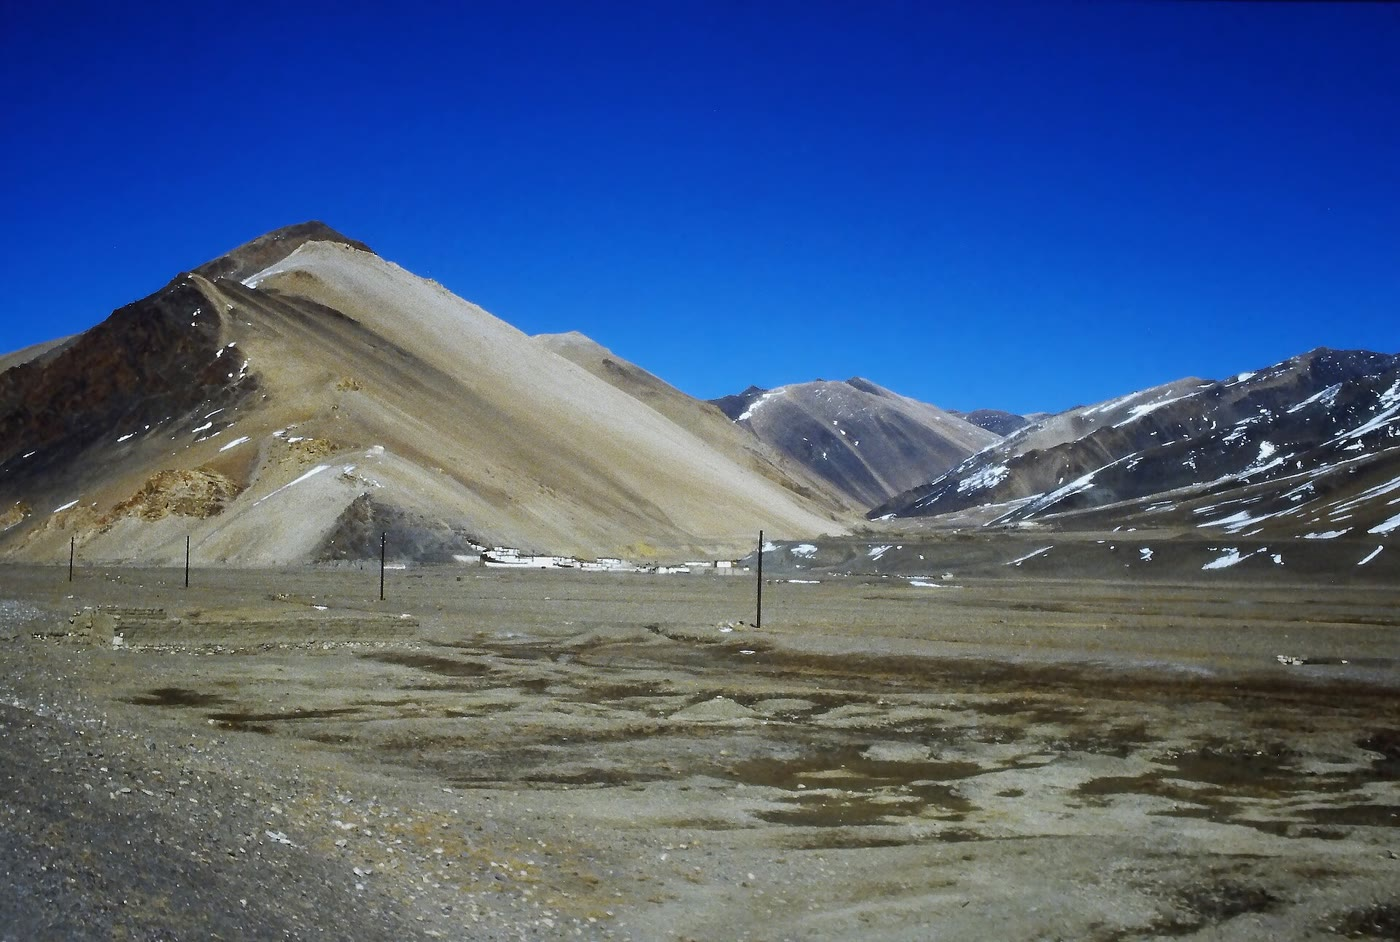
\includegraphics[width=0.66\linewidth]{images/book4/b2-14-tibet-plateau.jpg}
\par\smallskip{\small O Planalto Tibetano entre o Nepal e Shigatse: um piso plano de cascalho e
pastagem rala, com uma aldeia, entre montanhas nuas cobertas de tálus, o conjunto a mais de
quatro quilômetros acima do nível do mar.
Fotografia de Jan Kranendonk, 1987, CC BY-SA 4.0.}
\end{omfigure}
% ledger: data:b4-etopo-tibet

\subsection{O peso de um planalto}

Um planalto pesa sobre o seu entorno. Em cada profundidade até a base da sua raiz, uma coluna
sob o planalto está sob uma pressão maior do que uma coluna sob as terras baixas vizinhas;
só na profundidade de compensação as duas são iguais. A coluna alta empurra para fora.

\begin{proposition}[Energia potencial excedente de um planalto]\label{prop:b2:himalaya-andes:gpe}
Sob as hipóteses da \cref{prop:b2:himalaya-andes:airy}, com a gravidade $g$, a integral da
pressão litostática excedente da coluna do planalto em relação à coluna normal, do topo
do planalto à profundidade de compensação na base da sua raiz $r$, é
\[
  \Delta F = \rho_c g h \left(H + \frac{h}{2} + \frac{r}{2}\right) .
\]
Ela é a energia potencial gravitacional excedente da coluna do planalto por unidade de área, e a
força por unidade de comprimento da borda do planalto com a qual o planalto empurra o seu
entorno.
\end{proposition}

\begin{proof}
Meça-se a profundidade $z$ para baixo a partir do nível do mar. Na coluna do planalto, a pressão é $p_1 =
\rho_c g (z + h)$ de $z = -h$ a $L = H + r$. Na coluna normal, ela é nula acima do nível do
mar, $\rho_c g z$ na crosta, e $\rho_c g H + \rho_m g (z - H)$ abaixo. A diferença $p_1
- p_0$ sobe de 0 em $z = -h$ a $\rho_c g h$ ao nível do mar; ela mantém esse valor através da
crosta normal, onde as duas colunas são crosta; abaixo de $z = H$ ela diminui linearmente, de
$(\rho_m - \rho_c) g$ por metro, e chega a zero em $L$, pois $(\rho_m - \rho_c) r = \rho_c
h$. A integral é a área desse trapézio: $\rho_c g h\,(h/2 + H + r/2)$. O trabalho realizado pelas
pressões quando as duas colunas trocam matéria lateralmente é essa integral, e é por isso que ela
mede ao mesmo tempo a energia e o empurrão.
\end{proof}

\begin{omfigure}
\centering
% figdata/bachelor-2/plateaus.py part pressure (h = 4.8 km, H = 35 km, 2700 and 3300 kg/m3)
\begin{tikzpicture}
\begin{axis}[width=0.62\linewidth, height=5.6cm, y dir=reverse, xmin=0, xmax=160, ymin=-12,
  ymax=60, xlabel={pressão excedente $p_1 - p_0$ (\unit{MPa})}, ylabel={profundidade abaixo do nível do mar
  (\unit{km})}, tick label style={font=\scriptsize}, label style={font=\small},
  xtick pos=bottom, ytick pos=left, clip=false]
\addplot[fill=omThm!20, draw=omThm, line width=1pt] table[x expr=\thisrow{p_high_MPa}-\thisrow{p_ref_MPa}, y=z_km] {figdata/out/bachelor-2-plateaus-pressure.dat} \closedcycle;
\draw[dashed] (axis cs:0,0) -- (axis cs:160,0);
\draw[dashed] (axis cs:0,35) -- (axis cs:160,35);
\draw[dashed] (axis cs:0,56.6) -- (axis cs:160,56.6);
\node[font=\scriptsize, anchor=north east] at (axis cs:160,0) {nível do mar};
\node[font=\scriptsize, anchor=north east] at (axis cs:160,35) {Moho normal, $H$};
\node[font=\scriptsize, anchor=south east] at (axis cs:160,56.6) {base da raiz, $H + r$};
\node[font=\scriptsize, anchor=west] at (axis cs:100,-8.4) {topo do planalto, $-h$};
\node[font=\scriptsize, align=center] at (axis cs:60,20) {área $= \Delta F$\\$\approx\qty{6.1e12}{N.m^{-1}}$};
\end{axis}
\end{tikzpicture}
\par\smallskip{\small A pressão litostática excedente de uma coluna de planalto em relação a uma coluna
normal, para $h = \qty{4.8}{km}$, $H = \qty{35}{km}$ e densidades de 2700 e
\qty{3300}{kg.m^{-3}}: ela sobe através do planalto, fica em $\rho_c g h = \qty{127}{MPa}$
através da crosta normal, e cai a zero na base da raiz. A área sombreada é a
energia potencial excedente da \cref{prop:b2:himalaya-andes:gpe}.}
\end{omfigure}
% values (plateaus.py): tibet_gpe 6.12179e12 N/m for h = 4.8

Para o Tibete, $r = 4.5 \times 4.8 = \qty{21.6}{km}$ e $\Delta F = 2700 \times 9.8 \times 4800
\times (35000 + 2400 + 10800) \approx \qty{6.1e12}{N.m^{-1}}$. Distribuída sobre uma litosfera
de \qty{100}{km} de espessura, ela corresponde a uma tensão excedente média de cerca de \qty{60}{MPa}, da ordem das
tensões que rompem as rochas. Um planalto tão pesado já não pode simplesmente subir: ele tende a se espalhar.

\begin{definition}[Colapso gravitacional]\label{def:b2:himalaya-andes:collapse}
O \emph{colapso gravitacional}\index{colapso gravitacional (de um orógeno)} de um \omterm{def:b2:alpine-orogen:orogen}{orógeno}
é o espalhamento de sua crosta espessada sob seu próprio peso, por extensão das regiões
altas e escoamento ou cavalgamento para fora nas bordas, movido pela energia potencial excedente das
colunas espessadas.
\end{definition}

O Tibete está sendo estirado enquanto a Índia ainda o empurra. Através do sul do Tibete, riftes
norte--sul cortam o planalto e acomodam uma extensão leste--oeste: cerca de $9 \pm \qty{2}{mm}$ por ano ao
todo entre \ang{81} e \ang{92}~L, $1.3 \pm \qty{0.3}{mm}$ por ano só no rifte de Yadong--Gulu;
ao norte do Nepal, as estações GPS mostram o sul do planalto se estirando a cerca de
\num{12e-9} por ano. Os terremotos contam a mesma história: falhamento de cavalgamento e \omterm{def:b2:himalaya-andes:thickening}{espessamento crustal}
dominam as terras mais baixas em torno do planalto, falhamento transcorrente e normal o seu interior.
Por que ele se estende é debatido. No planalto oriental, a extensão foi lida como \omterm{def:b2:himalaya-andes:collapse}{colapso
gravitacional} movido pelo peso do planalto; no sul, outros a ligam à forma curva
do arco do Himalaia, ao longo do qual os cavalgamentos divergem, ou à Índia deslizando por baixo.
% ledger: wang21:rifts, ader12:extension

\subsection{Escapar para os lados}

\begin{definition}[Extrusão lateral]\label{def:b2:himalaya-andes:extrusion}
A \emph{extrusão lateral}\index{extrusão lateral} (tectônica de escape) é a expulsão de
blocos de crosta ou de litosfera para os lados de uma zona de colisão, ao longo de grandes falhas transcorrentes,
mais ou menos perpendicularmente à direção de convergência, em direção a um limite livre.
\end{definition}

A leste do Tibete, a Ásia não é apenas encurtada; ela é empurrada para o lado. Longas falhas transcorrentes
sinistrais, entre elas as falhas do Rio Vermelho e de Altyn Tagh, são lidas como tendo guiado o
escape para leste e para sudeste de grandes blocos, primeiro o bloco de Sunda, do Sudeste Asiático,
depois o Tibete e o sul da China, enquanto riftes e jovens bacias oceânicas se abriam em suas extremidades.
Experimentos nos quais um punção rígido era empurrado numa camada de massa de modelar produziram falhas assim;
modelos que tratavam a Ásia como uma lâmina viscosa contínua produziram, em vez disso, um espessamento amplo, sem
grandes falhas. O GPS sustenta o movimento de blocos: em relação à Sibéria estável, a bacia do Tarim
se move mais ou menos para o norte a cerca de \qty{14}{mm} por ano e o sul da China para lés-sudeste
a cerca de \qty{8}{mm} por ano. Quanto do avanço da Índia foi absorvido pelo espessamento e quanto
pela extrusão ainda é discutido.
% ledger: jiao23:extrusion

\section{Os Andes}\label{sec:b2:himalaya-andes:andes}

A placa de Nazca desce sob a América do Sul a cerca de \qty{72}{mm} por ano perto de
\ang{20}~S, para lés-nordeste, pelas velocidades angulares do NNR-MORVEL56. Nenhum continente
chegou, e no entanto os Andes Centrais carregam o segundo planalto mais alto da Terra.
% ledger: nnr56:poles
% values (plateaus.py): v_nazca_southamerica 72.52 mm/yr, azimuth 74.5

De oeste para leste, entre cerca de \ang{15} e \ang{27}~S, eles compreendem cinco zonas: o
\emph{antearco}; a \emph{Cordilheira Ocidental}, o arco vulcânico; o alto planalto, o
\emph{Altiplano} ao norte e a \emph{Puna} ao sul; a \emph{Cordilheira
Oriental}; e o \omterm{def:b2:alpine-orogen:ftb}{cinturão de dobras e cavalgamentos} de pele fina da \emph{zona Subandina}, que
passa à planície do Chaco. O perfil acima os atravessa a \ang{20}~S: a partir da fossa,
cujo nó mais profundo fica \qty{7.7}{km} abaixo do nível do mar a \ang{71.4}~O, a superfície sobe
mais de \qty{11}{km} em cerca de \qty{240}{km} até a borda do planalto a \ang{69.1}~O;
o planalto fica acima de \qty{3000}{m} por \qty{440}{km}, com uma
média de \qty{3760}{m}. A altura média é de \qty{3.7}{km} no Altiplano e de \qty{4.4}{km} na
Puna. Ao norte de \ang{23}~S, o Moho fica em geral a mais de \qty{60}{km}; sob o
Altiplano central, a crosta tem de 59 a \qty{64}{km} de espessura.
% ledger: gerbault05:andes, gerbault05:moho, data:b4-etopo-andes

\begin{omfigure}
\centering
\begin{tikzpicture}[x=0.56cm, y=0.38cm, font=\scriptsize]
% mantle background
\fill[gray!12] (0,-2.6) -- (5,-3.6) -- (8,-5.6) -- (10,-9.1) -- (12,-12.6) -- (13.2,-14.6) -- (26,-14.6)
  -- (26,-4.5) -- (20,-4.7) -- (17.5,-6.0) -- (15,-7.3) -- (11,-7.0) -- (9.5,-6.2) -- (8,-4) -- (5,-2)
  -- (0,-1) -- cycle;
% ocean water
\fill[blue!8] (0,0) -- (6.33,0) -- (5,-2) -- (0,-1) -- cycle;
% Nazca slab
\fill[gray!45] (0,-1) -- (5,-2) -- (8,-4) -- (10,-7.5) -- (12,-11) -- (14,-14.5) -- (13.2,-14.6)
  -- (12,-12.6) -- (10,-9.1) -- (8,-5.6) -- (5,-3.6) -- (0,-2.6) -- cycle;
% South American crust
\fill[orange!22] (5,-2) -- (8,1) -- (9,1.9) -- (10.2,2.0) -- (11,2.0) -- (15,2.0) -- (15.6,2.6) -- (16.8,2.4)
  -- (17.5,1.6) -- (20,0.6) -- (20.6,0.4) -- (26,0.3) -- (26,-4.5) -- (20,-4.7) -- (17.5,-6.0) -- (15,-7.3)
  -- (11,-7.0) -- (9.5,-6.2) -- (8,-4) -- cycle;
% Altiplano basin fill
\fill[yellow!45] (11,2.0) -- (15,2.0) -- (14.6,1.0) -- (11.4,1.0) -- cycle;
% surface line
\draw[line width=0.5pt] (0,-1) -- (5,-2) -- (8,1) -- (9,1.9) -- (10.2,2.0) -- (11,2.0) -- (15,2.0) -- (15.6,2.6)
  -- (16.8,2.4) -- (17.5,1.6) -- (20,0.6) -- (20.6,0.4) -- (26,0.3);
% arc volcanoes
\fill[red!60!black] (8.8,1.75) -- (9.2,2.9) -- (9.6,1.95) -- cycle;
\fill[red!60!black] (9.8,1.95) -- (10.2,2.8) -- (10.6,2.0) -- cycle;
\draw[red!60!black, decorate, decoration={snake, amplitude=0.6pt, segment length=4pt}] (10.8,-8.0) -- (9.9,1.6);
% Subandean decollement and splays
\draw[thick] (16.0,-1.2) -- (20.55,0.42);
\draw (17.4,-0.7) -- (17.85,1.45);
\draw (18.4,-0.35) -- (18.8,1.08);
\draw (19.4,0.0) -- (19.7,0.72);
% Moho
\draw[dashed] (8,-4) -- (9.5,-6.2) -- (11,-7.0) -- (15,-7.3) -- (17.5,-6.0) -- (20,-4.7) -- (26,-4.5);
% labels
\node at (2.6,-0.5) {Pacífico};
\node at (2.4,-2.2) {placa de Nazca};
\draw[-{Latex[length=1.6mm]}] (1.6,-2.8) -- (3.2,-3.0);
\node[anchor=south] (tr) at (4.3,0.9) {fossa};
\draw[->] (tr.south) -- (5,-1.8);
\node[anchor=south east] at (7.6,1.0) {antearco};
\node[anchor=south, align=center] at (9.7,3.0) {Cordilheira\\Ocidental (arco)};
\node[anchor=south] at (13,2.1) {Altiplano};
\node[anchor=south, align=center] at (16.4,2.7) {Cordilheira\\Oriental};
\node[anchor=south west] at (18.6,1.3) {Subandina};
\node[anchor=south] at (23.5,0.4) {planície do Chaco};
\node at (13,-3.2) {crosta espessa};
\node at (23.2,-2.0) {escudo brasileiro};
\node[anchor=north] at (23.2,-4.6) {Moho};
\node at (14.2,-9.6) {cunha mantélica};
\node at (21,-10) {manto};
\node[rotate=-50] at (12.75,-12.9) {laje};
\draw[-{Latex[length=2mm]}] (1.2,4.6) -- (0.2,4.6);
\node[anchor=south] at (0.7,4.6) {O};
\draw[-{Latex[length=2mm]}] (24.8,4.6) -- (25.8,4.6);
\node[anchor=south] at (25.3,4.6) {L};
\end{tikzpicture}
\par\smallskip{\small Uma seção esquemática através dos Andes Centrais perto de \ang{20}~S (fora de
escala). A placa de Nazca afunda sob o antearco; o \omterm{def:b2:magma-emplacement:magma}{magma} sobe da cunha mantélica (linha
ondulada) até o arco da Cordilheira Ocidental; o Altiplano, com seu espesso preenchimento de bacia, fica
entre as duas cordilheiras, sobre uma crosta de cerca de \qty{60}{km} de espessura; o cinturão
Subandino, de pele fina, cavalga para leste sobre o escudo brasileiro.}
\end{omfigure}
% ledger: gerbault05:andes, gerbault05:moho

\subsection{Como a crosta ficou espessa}

De onde veio a crosta extra do Altiplano? O primeiro candidato é o encurtamento:
comprima-se uma faixa de crosta e ela se espessa, conservando a área de sua seção transversal.

\begin{proposition}[Espessamento por encurtamento]\label{prop:b2:himalaya-andes:shortening}
Seja uma crosta de espessura uniforme $H$ encurtada, sem ganho nem perda de rocha, numa crosta
de espessura $T$ sobre uma largura $W$, a seção permanecendo paralela ao encurtamento. Sua
largura original era $W_0 = W T/H$, e o encurtamento é
\[
  S = W_0 - W = W\,\frac{T - H}{H} .
\]
\end{proposition}

\begin{proof}
A área da seção transversal da crosta se conserva, como no balanço de área da
\cref{prop:b2:alpine-orogen:balance}: $W_0 H = W T$. Logo $W_0 = WT/H$ e $S = W_0 - W =
W(T - H)/H$.
\end{proof}

A \ang{20}~S o planalto tem cerca de \qty{440}{km} de largura; se sua crosta, com cerca de \qty{60}{km} de espessura,
tinha outrora \qty{35}{km}, o encurtamento necessário é de $440 \times 25/35 \approx \qty{314}{km}$.
\omterm{def:b2:alpine-orogen:balanced}{Seções balanceadas} perto de 16--\ang{21}~S encontram cerca de \qty{50}{km} de encurtamento no Altiplano
e mais de \qty{200}{km} na zona Subandina desde o Oligoceno. Os volumes crustais
calculados a partir do encurtamento ficam cerca de \qty{20}{\percent} abaixo dos calculados a partir da profundidade
do Moho. Parte da diferença pode vir de hipóteses erradas, sobre a espessura inicial ou
sobre a natureza do Moho sísmico; parte pode ser crosta acrescentada de outras maneiras. Uma compilação perto de
\ang{21}~S atribui ao encurtamento tectônico pelo menos \qty{55}{\percent} da raiz, à
hidratação da cunha mantélica do antearco até \qty{20}{\percent}, e à adição magmática e à
erosão tectônica apenas cerca de \qty{5}{\percent}. A rocha também pode se deslocar dentro do cinturão:
diferenças de espessura crustal criam diferenças de energia potencial, como no Tibete, e
estas podem levar a crosta inferior quente a escoar do espesso para o fino.
% ledger: gerbault05:andes, gerbault05:volume, gerbault05:moho, data:b4-etopo-andes

\begin{omfigure}
\centering
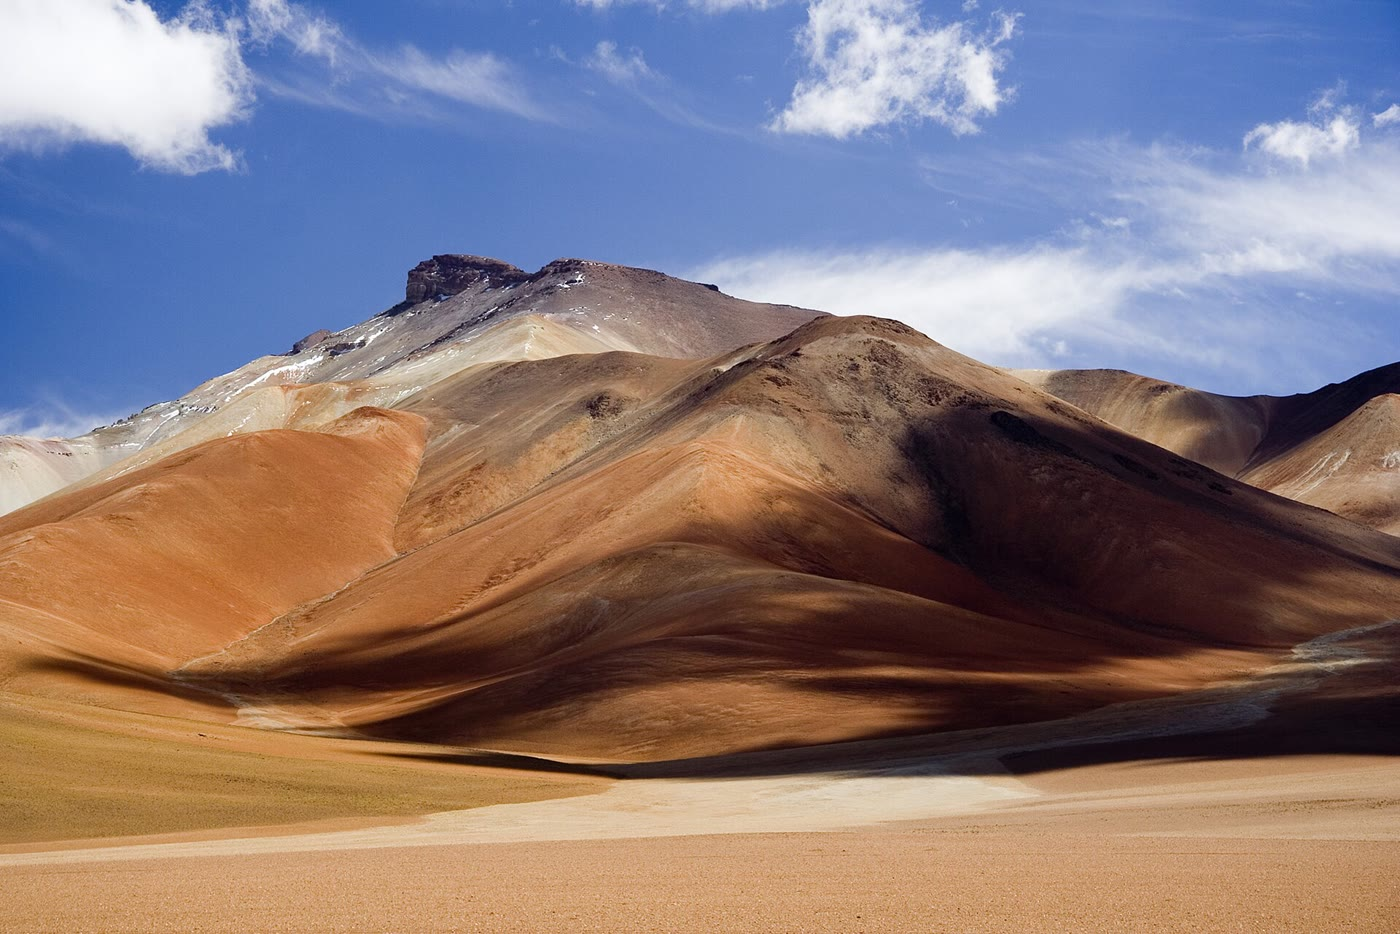
\includegraphics[width=0.66\linewidth]{images/book4/b2-14-altiplano.jpg}
\par\smallskip{\small O Altiplano boliviano: uma planície de areia e cascalho ao pé de
colinas nuas coloridas de vermelho, ocre e cinza por suas rochas. Fotografia de Luca Galuzzi, 2006, CC BY-SA 2.5.}
\end{omfigure}
% ledger: gerbault05:andes

\subsection{Lajes horizontais e raízes perdidas}

O ângulo da laje não é fixo, e isso importa na superfície.

\begin{definition}[Subducção horizontal]\label{def:b2:himalaya-andes:flat-slab}
A \emph{subducção horizontal}\index{subducção horizontal} é uma subducção na qual a laje,
depois de sua primeira descida, corre quase horizontalmente sob a placa cavalgante por centenas
de quilômetros antes de voltar a afundar.
\end{definition}

Ao longo dos Andes, dois segmentos da laje de Nazca são horizontais hoje, o segmento peruano, horizontal
desde cerca de \qty{15}{Ma}, e o segmento pampeano, desde cerca de \qty{18}{Ma}. Acima deles não há
vulcões ativos. Quando a laje pampeana se horizontalizou, o arco se deslocou para o interior e emitiu
menos lava; acima dos segmentos horizontais, ele silenciou. A distância arco--fossa do volume do primeiro ano
explica o deslocamento para o interior: quanto mais suave a laje sob o arco, mais longe da fossa ela
atinge a profundidade na qual a cunha funde; e uma laje que fica horizontal acima dessa profundidade não deixa
nenhuma cunha mantélica quente para fundir.
% ledger: gauthier24:flat

\begin{definition}[Delaminação litosférica]\label{def:b2:himalaya-andes:delamination}
A \emph{delaminação litosférica}\index{delaminação litosférica} é o destacamento e o
afundamento na astenosfera da parte inferior de uma litosfera espessada, seu manto
litosférico e às vezes uma crosta inferior densa, substituídos por astenosfera quente.
\end{definition}

A delaminação foi proposta sob a Puna meridional, entre \ang{24} e \ang{27}~S,
há cerca de 2 a \qty{3}{Ma}, onde jovens lavas máficas irromperam; e, ao longo do planalto, variações
de espessura crustal e de altitude foram ligadas a um manto litosférico já removido
sob o Altiplano meridional e ainda não completamente sob o Altiplano central. Perder uma
tampa mantélica densa torna a coluna restante mais leve: a superfície sobe sem nenhum
encurtamento adicional. A Puna fica cerca de \qty{1}{km} mais alta que o Altiplano sobre uma crosta cerca de
\qty{11}{km} mais fina, um contraste que exige ou uma crosta mais leve na Puna ou um manto mais leve
abaixo dela.
% ledger: gerbault05:delamination, gerbault05:moho

\section{Dois cinturões comparados}\label{sec:b2:himalaya-andes:compared}

Os dois planaltos se parecem de longe e diferem em quase todo o resto, como reúne a tabela
abaixo.

\begin{omfigure}
\centering\small
\begin{tabular}{>{\raggedright\arraybackslash}p{0.2\linewidth}|>{\raggedright\arraybackslash}p{0.34\linewidth}|>{\raggedright\arraybackslash}p{0.34\linewidth}}
 & Himalaia e Tibete & Andes Centrais \\ \hline
motor & continente contra continente depois do fechamento do oceano & placa oceânica afundando sob um continente \\
eixo & sutura com \omterm{def:b2:alpine-orogen:ophiolite}{ofiolitos} & arco vulcânico acima da laje \\
magmatismo & fundidos crustais: \omterm{def:b2:crustal-melting:leucogranite}{leucogranitos} & andesitos de arco; lavas máficas onde a litosfera foi perdida \\
convergência & cerca de \qty{45}{mm} por ano, metade absorvida na cadeia & cerca de \qty{72}{mm} por ano, consumidos sobretudo pela subducção \\
grandes terremotos & no MHT, Assam 1950, $M_w \approx 8.5$ & na interface de subducção, Chile 1960, $M_w$ 9.5 \\
planalto & média de \qty{4.8}{km} sobre \qty{1180}{km}; crosta de 70--\qty{75}{km} & média de \qty{3.8}{km} sobre \qty{440}{km}; crosta de cerca de \qty{60}{km} \\
tectônica do planalto & extensão leste--oeste, extrusão & encurtamento nos flancos; delaminação proposta \\
antepaís & antefossa indo-gangética e \omterm{def:b2:alpine-orogen:foreland}{molassa} das Siwalik & cinturão Subandino e planície do Chaco \\
\end{tabular}
\par\smallskip{\small Os dois cinturões lado a lado; as fontes são citadas nas seções acima,
e o terremoto do Chile é o maior registrado desde 1900.}
\end{omfigure}
% ledger: lave00:setting, lave00:siwaliks, weinberg16:himalaya, ader12:mht, ader12:quakes, usgs:largest, gerbault05:andes, gerbault05:moho, gerbault05:delamination, nnr56:poles, data:b4-etopo-tibet, data:b4-etopo-andes, cattin01:crust, wang21:rifts, jiao23:extrusion

A diferença mais profunda está no que desce. Nos Andes, a placa oceânica continua afundando, e
a maior parte da convergência, cerca de \qty{72}{mm} por ano, é consumida na fossa; encurtar a
placa superior em \qty{310}{km} ao longo de uns 30 milhões de anos tomaria apenas cerca de \qty{10}{mm} por
ano dela. No Himalaia, nada leve pode afundar por muito tempo, e a convergência é gasta em
empilhar, espessar e empurrar a Ásia para o lado. Os dois cinturões criam planaltos porque uma crosta espessa
é uma crosta alta; os dois planaltos param de subir quando seu próprio peso equilibra o empurrão nas suas
bordas, e então se espalham.
% ledger: nnr56:poles, gerbault05:andes, ader12:mht, jiao23:extrusion

\section{Que altura pode ter uma montanha?}\label{sec:b2:himalaya-andes:heights}

O cume mais alto, o Everest, fica a \qty{8848.86}{m} acima do nível do mar segundo o levantamento conjunto
anunciado em 2020. Por que não vinte quilômetros? Um limite grosseiro vem da resistência da rocha.

\begin{proposition}[Um limite de altura pela resistência da rocha]\label{prop:b2:himalaya-andes:height}
Uma coluna de rocha de densidade $\rho$ elevada a uma altura $h$ acima do seu entorno, sem
apoio lateral acima do nível dele, suporta em seu pé uma tensão vertical $\rho g h$ e uma
tensão horizontal nula em seus lados livres, logo uma tensão diferencial $\rho g h$. Se a
rocha rompe sob a tensão diferencial $\sigma_d$, a coluna só se mantém de pé se $h < \sigma_d/(\rho
g)$.
\end{proposition}

\begin{proof}
No pé da coluna, a tensão vertical é o peso da rocha acima por unidade de área,
$\rho g h$. Os lados são livres, de modo que a tensão horizontal ali é nula. A tensão diferencial
é a diferença entre a maior e a menor tensão principal, aqui $\rho g h - 0$.
A ruptura só é evitada se ela ficar abaixo de $\sigma_d$.
\end{proof}

Uma montanha real tem flancos inclinados que contêm seu núcleo, de modo que a tensão sob ela é
menor; como ordem de grandeza, tome-se a metade, $\rho g h/2$. Para o Everest, $2700 \times 9.8
\times 8849/2 \approx \qty{117}{MPa}$. A lei de Byerlee do volume do primeiro ano põe a resistência
por atrito da rocha numa falha sob uma tensão normal de \qty{200}{MPa} em $50 + 0.6 \times 200 =
\qty{170}{MPa}$: a mesma ordem. Uma montanha três vezes mais alta carregaria sua base muito além
do que a rocha suporta; ela romperia e se espalharia. Na Terra, cumes de oito a nove quilômetros
estão perto do limite, e um planalto, que se espalha muito antes de seus cumes romperem, se estabiliza
em cinco.
% ledger: tht:everest, byerlee:1975

\section*{Exercícios}\label{sec:b2:himalaya-andes:exercises}

Dados para os exercícios: $g = \qty{9.8}{m.s^{-2}}$; densidades da crosta e do manto
\qty{2700}{kg.m^{-3}} e \qty{3300}{kg.m^{-3}}, salvo indicação contrária; crosta normal $H =
\qty{35}{km}$.

\begin{exercise}[$\star$]\label{exo:b2:himalaya-andes:1}
Um planalto fica a uma altitude média de \qty{3.0}{km}. Usando a
\cref{prop:b2:himalaya-andes:airy}, calcule (a) sua raiz de Airy, (b) sua espessura crustal.
(c) Quanto o elevariam \qty{10}{km} a mais de crosta?
\end{exercise}

\begin{exercise}[$\star$]\label{exo:b2:himalaya-andes:2}
Uma travessia do Himalaia do Nepal vai da planície do Ganges ao Planalto Tibetano.
(a) Liste, em ordem, as unidades que ela atravessa e as falhas que as separam. (b) Que falha
é uma falha normal? (c) Como varia o grau metamórfico para o norte até a sequência do Alto
Himalaia, e depois acima dela?
\end{exercise}

\begin{exercise}[$\star$]\label{exo:b2:himalaya-andes:3}
No Nepal central, um terraço fluvial abandonado há \qty{9.2}{kyr} foi encurtado em
\qty{196.5}{m} através das dobras do Cavalgamento Frontal Principal. (a) Calcule a taxa média de encurtamento
em milímetros por ano. (b) Compare-a com a convergência GPS através da cadeia,
\qty{17.8}{mm} por ano. (c) O que a concordância diz sobre as falhas ao norte do MFT?
\end{exercise}

\begin{exercise}[$\star$]\label{exo:b2:himalaya-andes:4}
Classifique cada observação como de \omterm{def:b2:himalaya-andes:types}{orógeno de colisão}, de \omterm{def:b2:himalaya-andes:types}{orógeno de tipo andino} ou dos dois: (a) uma sutura marcada
por \omterm{def:b2:alpine-orogen:ophiolite}{ofiolitos}; (b) uma linha de vulcões andesíticos ativos; (c) \omterm{def:b2:crustal-melting:leucogranite}{leucogranitos} fundidos a partir da
crosta; (d) uma fossa oceânica profunda ao longo da frente; (e) uma \omterm{def:b2:alpine-orogen:foreland}{bacia de antepaís} com \omterm{def:b2:alpine-orogen:foreland}{molassa};
(f) grandes terremotos numa falha de mergulho suave sob a cadeia.
\end{exercise}

\begin{exercise}[$\star\star$]\label{exo:b2:himalaya-andes:5}
A Índia se move a \qty{45}{mm} por ano em relação à Eurásia através do Himalaia; através do Nepal, a
própria cadeia absorve \qty{17.8}{mm} por ano no leste e \qty{20.5}{mm} por ano no oeste.
(a) Que fração da convergência a cadeia absorve em cada caso? (b) Para onde vai o
resto? (c) Em \qty{10}{Myr}, quanto encurtamento representa o restante?
\end{exercise}

\begin{exercise}[$\star\star$]\label{exo:b2:himalaya-andes:6}
(a) Usando a \cref{prop:b2:himalaya-andes:gpe}, calcule a energia potencial excedente do
Altiplano, de altitude média \qty{3.7}{km}. (b) Compare-a com a do Tibete, a \qty{4.8}{km}.
(c) Mostre que, para um planalto pouco elevado, $h \ll H$, $\Delta F$ cresce proporcionalmente a $h$, e, para um
planalto alto, mais depressa: o que isso implica para o crescimento de um planalto?
\end{exercise}

\begin{exercise}[$\star\star$]\label{exo:b2:himalaya-andes:7}
(a) Calcule $\rho g h/2$ sob o Everest, de \qty{8848.86}{m} de altura, com $\rho =
\qty{2700}{kg.m^{-3}}$. (b) Pela lei de Byerlee, $\tau = 0.85\,\sigma_n$ abaixo de \qty{200}{MPa} de
tensão normal e $\tau = \qty{50}{MPa} + 0.6\,\sigma_n$ acima; calcule $\tau$ para $\sigma_n =
100$ e \qty{200}{MPa}. (c) Que altura permitiria uma resistência de \qty{170}{MPa}, pela mesma
regra de ordem de grandeza?
\end{exercise}

\begin{exercise}[$\star\star$]\label{exo:b2:himalaya-andes:8}
Os riftes do sul do Tibete absorvem $9 \pm \qty{2}{mm}$ por ano de extensão leste--oeste entre
\ang{81} e \ang{92}~L. (a) Qual é a largura desse trecho a \ang{30}~N, com \qty{111.19}{km} por
grau sobre um meridiano? (b) Calcule a taxa média de deformação extensional, por ano e por segundo,
com seu intervalo. (c) Compare com os $(12.4 \pm 4.7) \times 10^{-9}$ por ano obtidos por GPS ao norte do Nepal.
\end{exercise}

\begin{exercise}[$\star\star$]\label{exo:b2:himalaya-andes:9}
O Cavalgamento Principal do Himalaia, travado sob o Nepal, acumula um déficit de momento de
\qty{6.6e19}{N.m} por ano; os terremotos dos últimos 500 anos liberaram apenas
\qty{0.9e19}{N.m} por ano. (a) Que fração do déficit eles liberaram? (b) Com $M_0 =
10^{1.5 M_w + 9.1}$\,\unit{N.m}, calcule o momento de um terremoto de $M_w$ 8.5. (c) Com que frequência
seriam necessários tais terremotos para equilibrar o déficit?
\end{exercise}

\begin{exercise}[$\star\star\star$]\label{exo:b2:himalaya-andes:10}
A Puna fica \qty{0.7}{km} mais alta que o Altiplano (4.4 contra \qty{3.7}{km}) sobre uma crosta
\qty{11}{km} mais fina. Tome-se a crosta do Altiplano com \qty{61.5}{km} de espessura e densidade de
\qty{2800}{kg.m^{-3}}, e um manto de \qty{3300}{kg.m^{-3}} sob os dois. (a) Escreva a
igualdade das massas das duas colunas acima de uma profundidade de compensação comum. (b) Encontre a
densidade que a crosta da Puna deve ter se só a crosta compensar a diferença. (c) Compare
com os 150 a \qty{200}{kg.m^{-3}} citados, e diga o que mais poderia explicar o contraste.
\end{exercise}

\begin{exercise}[$\star\star\star$]\label{exo:b2:himalaya-andes:11}
A frente vulcânica fica onde o topo da laje está a \qty{105}{km} de profundidade. (a) Para uma laje
mergulhando uniformemente a \ang{30}, calcule a distância arco--fossa com a fórmula do volume do primeiro
ano. (b) A laje agora mergulha a \ang{30} até \qty{90}{km}, depois a apenas \ang{4}: calcule
a nova distância e o deslocamento do arco para o interior. (c) O que acontece com o arco se a laje se horizontaliza
a \qty{95}{km} de profundidade e fica assim por \qty{300}{km}?
\end{exercise}

\begin{exercise}[$\star\star\star$]\label{exo:b2:himalaya-andes:12}
A erosão remove cerca de \qty{300}{km^3} de rocha por quilômetro de Himalaia por milhão de anos.
A Índia traz uma crosta de \qty{37.5}{km} de espessura a \qty{21}{mm} por ano. (a) Quanta crosta por
quilômetro de cadeia por milhão de anos entra no cinturão? (b) Que fração a erosão remove?
(c) Onde pode estar o resto?
\end{exercise}

\begin{problem}[{Problema de fim de semana --- dois planaltos}]\label{pb:b2:himalaya-andes:1}
Os perfis em faixa deste capítulo dão a altitude média dos nós através do Tibete
(\qtyrange{86}{90}{\degree} L) e através dos Andes Centrais (\qtyrange{19}{21}{\degree} S).
Amostrados a cada \ang{1.5} de latitude e a cada grau de longitude, arredondados a \qty{10}{m}, eles
dão o seguinte. Salvo indicação contrária, $g = \qty{9.8}{m.s^{-2}}$, $\rho_c = \qty{2700}{kg.m^{-3}}$,
$\rho_m = \qty{3300}{kg.m^{-3}}$ e a crosta normal tem $H = \qty{35}{km}$ de espessura.

\smallskip
\begin{center}\small
\begin{tabular}{l|ccccccccc}
latitude (\unit{\degree} N) & 26.5 & 28.0 & 29.5 & 31.0 & 32.5 & 34.0 & 35.5 & 37.0 & 38.5 \\ \hline
altitude média (\unit{m}) & 70 & 5000 & 5030 & 4830 & 5020 & 5150 & 5050 & 4470 & 2210
\end{tabular}

\smallskip
\begin{tabular}{l|cccccccc}
longitude (\unit{\degree}) & $-71$ & $-70$ & $-69$ & $-68$ & $-67$ & $-66$ & $-65$ & $-64$ \\ \hline
altitude média (\unit{m}) & $-3310$ & 970 & 4150 & 3720 & 3740 & 4010 & 3030 & 1170
\end{tabular}
\end{center}
\smallskip

\noindent\textbf{Parte I --- Ler os perfis.}
\begin{enumerate}
\item Tomando como planalto as amostras acima de \qty{3000}{m}, calcule a altitude média do Tibete
$h_T$, arredondada a \qty{0.1}{km}.
\item Faça o mesmo para o Altiplano, $h_A$, e compare com a altura média de
\qty{3.7}{km} citada para o Altiplano e de \qty{4.4}{km} para a Puna.
\item Qual é a largura mínima de cada planalto, segundo as amostras (\qty{111.19}{km} por
grau de latitude; \qty{104.5}{km} por grau de longitude a \ang{20}~S)?
\item Calcule a inclinação média da frente do Himalaia entre \ang{26.5} e \ang{28.0}~N, em
porcentagem.
\item Por que o perfil andino é tão mais assimétrico que o tibetano?
\end{enumerate}

\noindent\textbf{Parte II --- Espessuras de Airy.}
\begin{enumerate}[resume]
\item Calcule a raiz de Airy e a espessura crustal $T_T$ do Tibete a partir de $h_T$.
\item Faça o mesmo para o Altiplano, $T_A$.
\item Compare com as espessuras sísmicas, de 70 a \qty{75}{km} sob o Tibete e de 59 a
\qty{64}{km} sob o Altiplano central. Que estimativa está mais longe?
\item Que densidade crustal tornaria a espessura de Airy do Tibete igual a \qty{72.5}{km}?
\item Que densidade daria \qty{61.5}{km} para o Altiplano?
\item Cite duas razões, além da densidade crustal, pelas quais um cálculo de Airy local pode
não reproduzir a raiz observada.
\item A crosta tem \qty{37.5}{km} de espessura sob a Índia e \qty{72.5}{km} sob o Tibete. Com um
contraste de densidade no Moho de \qty{370}{kg.m^{-3}}, estime com a placa de Bouguer, $\Delta g
= 2\pi G\,\Delta\rho\,t$, a anomalia de Bouguer da raiz do Tibete em relação à Índia, sendo $t$ a
espessura extra abaixo do nível do mar ($G = \qty{6.674e-11}{m^3.kg^{-1}.s^{-2}}$). Compare com a
diferença observada de \qty{460}{mGal}.
\end{enumerate}

\noindent\textbf{Parte III --- Encurtar o Altiplano.} A \ang{20}~S, o planalto tem
\qty{440}{km} de largura e sua crosta, cerca de \qty{60}{km} de espessura.
\begin{enumerate}[resume]
\item Usando a \cref{prop:b2:himalaya-andes:shortening}, calcule a largura restaurada e o
encurtamento necessário se a crosta tinha antes \qty{35}{km} de espessura.
\item As \omterm{def:b2:alpine-orogen:balanced}{seções balanceadas} dão cerca de \qty{50}{km} de encurtamento no Altiplano e
\qty{200}{km} na zona Subandina. Que fração do encurtamento necessário está faltando?
\item Se o encurtamento produziu apenas \qty{55}{\percent} da crosta extra, quanto encurtamento é
necessário?
\item O cinturão Subandino é de pele fina. Por que seu encurtamento ainda assim deve espessar a crosta
em algum lugar?
\item Suponha que os \qty{314}{km} da Parte III tenham se acumulado em \qty{30}{Myr}. Calcule a taxa
média, e a fração da convergência atual Nazca--América do Sul, \qty{72}{mm} por ano, que
ela representa.
\item Para onde vai o resto da convergência?
\end{enumerate}

\noindent\textbf{Parte IV --- O peso do Tibete.}
\begin{enumerate}[resume]
\item Usando a \cref{prop:b2:himalaya-andes:gpe} com $h_T$, calcule a energia potencial excedente
do Tibete por unidade de área.
\item Calcule-a para o Altiplano com $h_A$, e a razão entre as duas.
\item Distribua o $\Delta F$ do Tibete sobre uma litosfera de \qty{100}{km} de espessura: que tensão média
ele representa?
\item A extensão do sul do Tibete, \qty{9}{mm} por ano através de \qty{1060}{km}, corresponde a quanta
deformação por ano?
\item Por que o Tibete pode se estender de leste a oeste enquanto a Índia ainda o empurra para o norte?
\item Para resumir: dê a espessura crustal do Tibete calculada a partir de sua altitude média, arredondada
ao quilômetro, e a fração dos \qty{72.5}{km} sísmicos que ela explica.
\end{enumerate}
\end{problem}
